% Options for packages loaded elsewhere
\PassOptionsToPackage{unicode}{hyperref}
\PassOptionsToPackage{hyphens}{url}
\PassOptionsToPackage{dvipsnames,svgnames,x11names}{xcolor}
%
\documentclass[
  letterpaper,
  DIV=11,
  numbers=noendperiod]{scrartcl}

\usepackage{amsmath,amssymb}
\usepackage{iftex}
\ifPDFTeX
  \usepackage[T1]{fontenc}
  \usepackage[utf8]{inputenc}
  \usepackage{textcomp} % provide euro and other symbols
\else % if luatex or xetex
  \usepackage{unicode-math}
  \defaultfontfeatures{Scale=MatchLowercase}
  \defaultfontfeatures[\rmfamily]{Ligatures=TeX,Scale=1}
\fi
\usepackage{lmodern}
\ifPDFTeX\else  
    % xetex/luatex font selection
\fi
% Use upquote if available, for straight quotes in verbatim environments
\IfFileExists{upquote.sty}{\usepackage{upquote}}{}
\IfFileExists{microtype.sty}{% use microtype if available
  \usepackage[]{microtype}
  \UseMicrotypeSet[protrusion]{basicmath} % disable protrusion for tt fonts
}{}
\makeatletter
\@ifundefined{KOMAClassName}{% if non-KOMA class
  \IfFileExists{parskip.sty}{%
    \usepackage{parskip}
  }{% else
    \setlength{\parindent}{0pt}
    \setlength{\parskip}{6pt plus 2pt minus 1pt}}
}{% if KOMA class
  \KOMAoptions{parskip=half}}
\makeatother
\usepackage{xcolor}
\setlength{\emergencystretch}{3em} % prevent overfull lines
\setcounter{secnumdepth}{-\maxdimen} % remove section numbering
% Make \paragraph and \subparagraph free-standing
\makeatletter
\ifx\paragraph\undefined\else
  \let\oldparagraph\paragraph
  \renewcommand{\paragraph}{
    \@ifstar
      \xxxParagraphStar
      \xxxParagraphNoStar
  }
  \newcommand{\xxxParagraphStar}[1]{\oldparagraph*{#1}\mbox{}}
  \newcommand{\xxxParagraphNoStar}[1]{\oldparagraph{#1}\mbox{}}
\fi
\ifx\subparagraph\undefined\else
  \let\oldsubparagraph\subparagraph
  \renewcommand{\subparagraph}{
    \@ifstar
      \xxxSubParagraphStar
      \xxxSubParagraphNoStar
  }
  \newcommand{\xxxSubParagraphStar}[1]{\oldsubparagraph*{#1}\mbox{}}
  \newcommand{\xxxSubParagraphNoStar}[1]{\oldsubparagraph{#1}\mbox{}}
\fi
\makeatother


\providecommand{\tightlist}{%
  \setlength{\itemsep}{0pt}\setlength{\parskip}{0pt}}\usepackage{longtable,booktabs,array}
\usepackage{calc} % for calculating minipage widths
% Correct order of tables after \paragraph or \subparagraph
\usepackage{etoolbox}
\makeatletter
\patchcmd\longtable{\par}{\if@noskipsec\mbox{}\fi\par}{}{}
\makeatother
% Allow footnotes in longtable head/foot
\IfFileExists{footnotehyper.sty}{\usepackage{footnotehyper}}{\usepackage{footnote}}
\makesavenoteenv{longtable}
\usepackage{graphicx}
\makeatletter
\newsavebox\pandoc@box
\newcommand*\pandocbounded[1]{% scales image to fit in text height/width
  \sbox\pandoc@box{#1}%
  \Gscale@div\@tempa{\textheight}{\dimexpr\ht\pandoc@box+\dp\pandoc@box\relax}%
  \Gscale@div\@tempb{\linewidth}{\wd\pandoc@box}%
  \ifdim\@tempb\p@<\@tempa\p@\let\@tempa\@tempb\fi% select the smaller of both
  \ifdim\@tempa\p@<\p@\scalebox{\@tempa}{\usebox\pandoc@box}%
  \else\usebox{\pandoc@box}%
  \fi%
}
% Set default figure placement to htbp
\def\fps@figure{htbp}
\makeatother

\usepackage{fvextra}
\DefineVerbatimEnvironment{Highlighting}{Verbatim}{breaklines,commandchars=\\\{\}}
\DefineVerbatimEnvironment{OutputCode}{Verbatim}{breaklines,commandchars=\\\{\}}
\KOMAoption{captions}{tableheading}
\makeatletter
\@ifpackageloaded{caption}{}{\usepackage{caption}}
\AtBeginDocument{%
\ifdefined\contentsname
  \renewcommand*\contentsname{Table of contents}
\else
  \newcommand\contentsname{Table of contents}
\fi
\ifdefined\listfigurename
  \renewcommand*\listfigurename{List of Figures}
\else
  \newcommand\listfigurename{List of Figures}
\fi
\ifdefined\listtablename
  \renewcommand*\listtablename{List of Tables}
\else
  \newcommand\listtablename{List of Tables}
\fi
\ifdefined\figurename
  \renewcommand*\figurename{Figure}
\else
  \newcommand\figurename{Figure}
\fi
\ifdefined\tablename
  \renewcommand*\tablename{Table}
\else
  \newcommand\tablename{Table}
\fi
}
\@ifpackageloaded{float}{}{\usepackage{float}}
\floatstyle{ruled}
\@ifundefined{c@chapter}{\newfloat{codelisting}{h}{lop}}{\newfloat{codelisting}{h}{lop}[chapter]}
\floatname{codelisting}{Listing}
\newcommand*\listoflistings{\listof{codelisting}{List of Listings}}
\makeatother
\makeatletter
\makeatother
\makeatletter
\@ifpackageloaded{caption}{}{\usepackage{caption}}
\@ifpackageloaded{subcaption}{}{\usepackage{subcaption}}
\makeatother

\usepackage{bookmark}

\IfFileExists{xurl.sty}{\usepackage{xurl}}{} % add URL line breaks if available
\urlstyle{same} % disable monospaced font for URLs
\hypersetup{
  pdftitle={RPG Assessment for Ellice Huang},
  colorlinks=true,
  linkcolor={blue},
  filecolor={Maroon},
  citecolor={Blue},
  urlcolor={Blue},
  pdfcreator={LaTeX via pandoc}}


\title{RPG Assessment for Ellice Huang}
\author{}
\date{}

\begin{document}
\maketitle


\subsection{TASK 1}\label{task-1}

\emph{Writing a function that filters and aggregates data by card family
and customer segment, based on a date and customer age range. Function
is called for age 28-44 and date May 10th - Jul 16th (inclusive) below.}

\begin{longtable}[]{@{}llllll@{}}
\toprule\noalign{}
& Card\_Family & Customer\_Segment & \multicolumn{3}{l@{}}{%
Transaction\_Value} \\
& & & count & mean & std \\
\midrule\noalign{}
\endhead
\bottomrule\noalign{}
\endlastfoot
0 & Gold & Diamond & 159 & 25947.490566 & 14295.469532 \\
1 & Gold & Gold & 110 & 24850.972727 & 13211.350331 \\
2 & Gold & Platinum & 60 & 22826.933333 & 14499.972092 \\
3 & Platinum & Diamond & 91 & 23105.197802 & 13891.667734 \\
4 & Platinum & Gold & 65 & 24459.815385 & 13725.743636 \\
5 & Platinum & Platinum & 65 & 24620.600000 & 14958.461580 \\
6 & Premium & Diamond & 195 & 23435.748718 & 15538.776861 \\
7 & Premium & Gold & 136 & 23741.492647 & 14526.895788 \\
8 & Premium & Platinum & 93 & 25273.182796 & 14595.783222 \\
\end{longtable}

\subsection{TASK 2}\label{task-2}

\emph{Building a logistic regression model using the statsmodels package
to predict fraud using transaction value, value as a share of limit,
age, card family, customer segment, and transaction segment; no cross
validation.}

The results of a logistic model using transaction value, credit limit
share, age, card family, customer segment, and transaction segment are
displayed below.

Here are a few takeaways from this model:

\begin{itemize}
\tightlist
\item
  There are likely other factors that should be accounted for in
  predicting fraud. The \emph{R-squared value} of 0.1687 suggests that
  only about 16.87\% of the variability in the fraud variable can be
  explained by the model.
\item
  Higher \emph{credit limit share} values are associated with increased
  odds of fraud, by about 6\% (exp(0.0595)) per unit of increase in
  limit share. This coefficient is statistically significant
  (p\textless0.001).
\item
  In terms of \emph{age}, a statistically significant positive
  coefficient (p\textless0.1) suggests that for each additional year of
  age, the odds of being associated with a fradulent transaction
  increases by about 0.8\%.
\item
  In terms of \emph{card family}, compared to the gold family, platinum
  card transactions are associated with lower odds of being fraudulent
  by 96\% (statistically significant with p\textless.001) while premium
  card transactions are associated with substantially higher odds of
  being fraudulent by 227\% (p\textless.001).
\item
  In terms of \emph{customer segment}, compared to the diamond group,
  gold customer transactions are associated with lower odds of being
  fraud by about 17\% (p\textless.001). The platinum segment coefficient
  is not statistically significant, suggesting no strong difference in
  odds.
\item
  Finally, none of the \emph{transaction segment} coefficients are
  statistically significiant, indicating that these segments are not
  helpful indicators in predicting the likelihood of fraud.
\end{itemize}

\begin{center}
\begin{tabular}{lclc}
\toprule
\textbf{Dep. Variable:}              &   Fraud\_Flag    & \textbf{  No. Observations:  } &    10000    \\
\textbf{Model:}                      &      Logit       & \textbf{  Df Residuals:      } &     9978    \\
\textbf{Method:}                     &       MLE        & \textbf{  Df Model:          } &       21    \\
\textbf{Date:}                       & Mon, 30 Dec 2024 & \textbf{  Pseudo R-squ.:     } &   0.1687    \\
\textbf{Time:}                       &     15:01:35     & \textbf{  Log-Likelihood:    } &   -4849.3   \\
\textbf{converged:}                  &       True       & \textbf{  LL-Null:           } &   -5833.6   \\
\textbf{Covariance Type:}            &    nonrobust     & \textbf{  LLR p-value:       } &    0.000    \\
\bottomrule
\end{tabular}
\begin{tabular}{lcccccc}
                                     & \textbf{coef} & \textbf{std err} & \textbf{z} & \textbf{P$> |$z$|$} & \textbf{[0.025} & \textbf{0.975]}  \\
\midrule
\textbf{const}                       &      -1.6552  &        0.156     &   -10.589  &         0.000        &       -1.962    &       -1.349     \\
\textbf{Transaction\_Value}          &    2.497e-06  &     1.76e-06     &     1.423  &         0.155        &    -9.43e-07    &     5.94e-06     \\
\textbf{Limit\_Share}                &       0.0595  &        0.016     &     3.826  &         0.000        &        0.029    &        0.090     \\
\textbf{Age}                         &       0.0080  &        0.003     &     2.831  &         0.005        &        0.002    &        0.014     \\
\textbf{Card\_Family\_Platinum}      &      -3.2879  &        0.219     &   -14.995  &         0.000        &       -3.718    &       -2.858     \\
\textbf{Card\_Family\_Premium}       &       1.1844  &        0.057     &    20.709  &         0.000        &        1.072    &        1.297     \\
\textbf{Customer\_Segment\_Gold}     &      -0.1900  &        0.057     &    -3.357  &         0.001        &       -0.301    &       -0.079     \\
\textbf{Customer\_Segment\_Platinum} &      -0.0230  &        0.064     &    -0.360  &         0.719        &       -0.148    &        0.102     \\
\textbf{Transaction\_Segment\_SEG12} &       0.0733  &        0.133     &     0.550  &         0.582        &       -0.188    &        0.334     \\
\textbf{Transaction\_Segment\_SEG13} &      -0.0018  &        0.134     &    -0.014  &         0.989        &       -0.265    &        0.261     \\
\textbf{Transaction\_Segment\_SEG14} &      -0.0515  &        0.138     &    -0.372  &         0.710        &       -0.322    &        0.219     \\
\textbf{Transaction\_Segment\_SEG15} &       0.0737  &        0.133     &     0.552  &         0.581        &       -0.188    &        0.335     \\
\textbf{Transaction\_Segment\_SEG16} &      -0.2070  &        0.138     &    -1.501  &         0.133        &       -0.477    &        0.063     \\
\textbf{Transaction\_Segment\_SEG17} &       0.0573  &        0.135     &     0.426  &         0.670        &       -0.207    &        0.321     \\
\textbf{Transaction\_Segment\_SEG18} &      -0.1205  &        0.135     &    -0.892  &         0.372        &       -0.385    &        0.144     \\
\textbf{Transaction\_Segment\_SEG19} &      -0.1516  &        0.138     &    -1.096  &         0.273        &       -0.423    &        0.120     \\
\textbf{Transaction\_Segment\_SEG20} &       0.2471  &        0.132     &     1.870  &         0.061        &       -0.012    &        0.506     \\
\textbf{Transaction\_Segment\_SEG21} &       0.0630  &        0.135     &     0.467  &         0.641        &       -0.202    &        0.328     \\
\textbf{Transaction\_Segment\_SEG22} &       0.0428  &        0.135     &     0.316  &         0.752        &       -0.222    &        0.308     \\
\textbf{Transaction\_Segment\_SEG23} &       0.0966  &        0.133     &     0.729  &         0.466        &       -0.163    &        0.356     \\
\textbf{Transaction\_Segment\_SEG24} &       0.1300  &        0.134     &     0.969  &         0.333        &       -0.133    &        0.393     \\
\textbf{Transaction\_Segment\_SEG25} &      -0.0274  &        0.136     &    -0.201  &         0.841        &       -0.294    &        0.239     \\
\bottomrule
\end{tabular}
%\caption{Logit Regression Results}
\end{center}

\subsection{TASK 3}\label{task-3}

\emph{Implementing a lightGBM and logistic regression classification
algorithm using scikit-learn to predict fraud using Transaction Value,
Credit Limit, Age, and Card Family as features/predictors with 80/20
cross validation. Transactions calssified as fraud if they have a
greater than 0.25 (25\%) predicted probability.}

\subsubsection{Model 1: LGBM}\label{model-1-lgbm}

For this task, I chose to implement a LightGBM classification model. The
confusion matrix and classification report for the LGBM model are
displayed below. The AUC score for this model is 0.812.

\begin{longtable}[]{@{}lll@{}}
\toprule\noalign{}
& pred\_0 & pred\_1 \\
\midrule\noalign{}
\endhead
\bottomrule\noalign{}
\endlastfoot
actual\_0 & 1007 & 463 \\
actual\_1 & 134 & 396 \\
\end{longtable}

\begin{longtable}[]{@{}llllll@{}}
\toprule\noalign{}
& 0.0 & 1.0 & accuracy & macro avg & weighted avg \\
\midrule\noalign{}
\endhead
\bottomrule\noalign{}
\endlastfoot
precision & 0.882559 & 0.461001 & 0.7015 & 0.671780 & 0.770846 \\
recall & 0.685034 & 0.747170 & 0.7015 & 0.716102 & 0.701500 \\
f1-score & 0.771352 & 0.570194 & 0.7015 & 0.670773 & 0.718045 \\
support & 1470.000000 & 530.000000 & 0.7015 & 2000.000000 &
2000.000000 \\
\end{longtable}

\subsubsection{Model 2: Logistic
Regression}\label{model-2-logistic-regression}

The confusion matrix and classification report for the logit model are
displayed below. The AUC score for this model is 0.788.

\begin{longtable}[]{@{}lll@{}}
\toprule\noalign{}
& pred\_0 & pred\_1 \\
\midrule\noalign{}
\endhead
\bottomrule\noalign{}
\endlastfoot
actual\_0 & 1098 & 372 \\
actual\_1 & 177 & 353 \\
\end{longtable}

\begin{longtable}[]{@{}llllll@{}}
\toprule\noalign{}
& 0.0 & 1.0 & accuracy & macro avg & weighted avg \\
\midrule\noalign{}
\endhead
\bottomrule\noalign{}
\endlastfoot
precision & 0.861176 & 0.486897 & 0.7255 & 0.674037 & 0.761992 \\
recall & 0.746939 & 0.666038 & 0.7255 & 0.706488 & 0.725500 \\
f1-score & 0.800000 & 0.562550 & 0.7255 & 0.681275 & 0.737076 \\
support & 1470.000000 & 530.000000 & 0.7255 & 2000.000000 &
2000.000000 \\
\end{longtable}

\subsubsection{Metric evaluation table}\label{metric-evaluation-table}

The table below summarizes the evaluation metrics for the lgbm and
logistic models.

\begin{longtable}[]{@{}llll@{}}
\toprule\noalign{}
& metric & lgbm & logistic \\
\midrule\noalign{}
\endhead
\bottomrule\noalign{}
\endlastfoot
0 & precision & 0.461001 & 0.486897 \\
1 & recall & 0.747170 & 0.666038 \\
2 & f1 & 0.570194 & 0.562550 \\
3 & auc & 0.811617 & 0.787994 \\
4 & true negative & 1007.000000 & 1098.000000 \\
5 & false positive & 463.000000 & 372.000000 \\
6 & false negative & 134.000000 & 177.000000 \\
7 & true positive & 396.000000 & 353.000000 \\
\end{longtable}

\subsubsection{Metric evaluation plots}\label{metric-evaluation-plots}

Below the ROC and precision-recall curves for the lgbm and logistic
models are displayed.

\pandocbounded{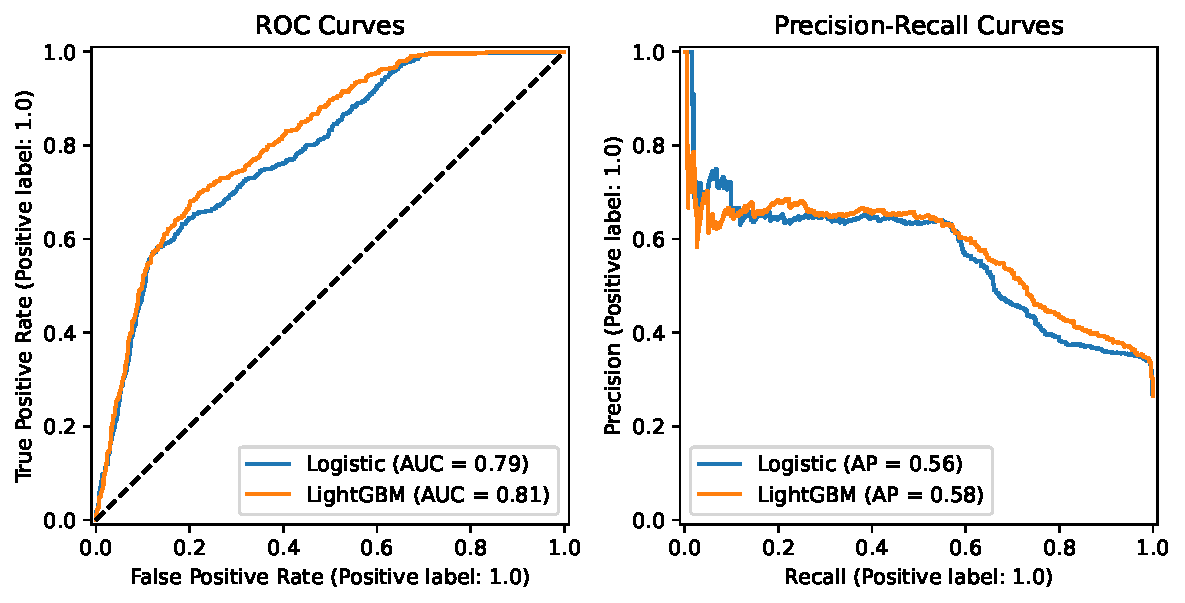
\includegraphics[keepaspectratio]{main_files/figure-pdf/cell-14-output-1.pdf}}

\subsection{TASK 4}\label{task-4}

\subsubsection{Model comparison}\label{model-comparison}

Based on my analysis, I conclude that a LightGBM model would be
preferable over a logistic regression model in a production setting.

It is important to note that I assume a credit card company's primary
goal is to minimize false negatives and prioritize recall over
precision. Missing actual fraudulent cases would be much more costly
than falsely flagging legitimate transactions. While false alarms can
inconvenience customers, this is of lower priority than overlooking
fraud, which would result in financial losses and reputational damage.

My conclusion is supported by the metrics table and plots above:

\begin{itemize}
\tightlist
\item
  The LGBM model has a substantially higher \emph{recall} score (0.75)
  than the logistic model (0.67), meaning that the LGBM model is able to
  capture a significant portion of fraudulent transactions.
\item
  While the logistic model has higher \emph{precision} (0.49) than the
  lgbm model (0.46), this difference is negligible compared to the
  significant difference in recall.
\item
  The \emph{precision-recall graph} visualizes the difference in
  precision and recall between the two models. The LGBM curve is
  slightly higher and pulled to the right, signifying that it
  outperforms the logistic model.
\item
  The \emph{F1 scores} are similar, with the LGBM model scoring slightly
  higher (.57 vs .56), suggesting both models are able to balance
  precision and recall.
\item
  The LGBM model also has a slightly higher \emph{AUC score} (.81
  vs.~.79), indicating the LGBM model is more accurate at distinguishing
  between the two classes. The \emph{ROC curves} visualize this, showing
  that for different classification thresholds, the LGBM model has
  better sensitivity and specificity on average.
\item
  Looking at the numbers more closely, the LGBM model is able to
  identify more true positives (396 vs 353 out of 530 total fraud
  cases). While the logistic model is able to limit more false positives
  (372 vs 463), I believe the LGBM's better ability to identify fraud
  makes it the better model for this setting.
\end{itemize}

Finally, LGBM is the better model in terms of large-scale performance
and scalability. A fraud classifier would have to handle a significant
amount of data, with millions of users and transactions. LGBM models
\href{https://www.nature.com/articles/s41598-022-20149-z?utm_source=chatgpt.com}{outperform}
logistic models and improve with larger sample sizes and datasets. They
have superior speed and efficiency, and exhibit efficient resource
utilization even as datasets grow.

To limit the false positive rate and improve customer satisfaction, I
would recommend adjusting the decision threshold for classifying fraud
cases, implementing additional verification steps for flagged
transactions, and developing user-friendly methods for customers to
verify whether flagged transactions are actually fraudulent.

\subsubsection{Experiment
recommendation}\label{experiment-recommendation}

The program described could be implemented as a randomized controlled
trial. To determine whether the anti-fraud program is effective, I
suggest the following strategy:

\begin{enumerate}
\def\labelenumi{\arabic{enumi}.}
\tightlist
\item
  Collect data over a minimum of 12-18 months to allow for enough time
  to detect fraudulent patterns and account for seasonal/holiday
  variations.
\item
  Collect all transaction information, including ID, date, merchant
  description, credit card information, amount, and whether the
  transaction was fraudulent.
\item
  Collect customer information, such as age, education level, credit
  score, income level, and residence zip code.
\item
  Collect information on outcome variables that indicate whether the
  program was effective. This includes the number of fraud cases, the
  company's financial losses due to fraud, customer complaints due to
  falsely flagged transactions, and the operational costs associated
  with the anti-fraud program, such as implementation or resource
  utilization. The company can also consider implementing surveys to
  gauge program impact on customer satisfaction.
\item
  Implement a series of regression models to analyze the differences in
  outcomes between treatment and control groups. The outcome variables
  would include financial losses, number of fraudulent cases, and
  customer satisfaction. The independent variable with the coefficient
  of interest is whether the transaction was treated with the anti-fraud
  program, and the remainder of the variables will serve as control
  variables.
\item
  Use the findings from the control variables to continually improve on
  the anti-fraud program. For example, the model may indicate that more
  fraudulent transactions occur during the holiday season, in particular
  zip codes, or higher age ranges.
\end{enumerate}

In order for the program to be deemed as effective, there would need to
be a statistically significant treatment effect indicating that cases in
the anti-fraud program were associated with less financial losses, less
fraudulent cases, and better customer satisfaction. Because this is a
randomized controlled trial, the treatment effect could be interpreted
as a direct causal effect of the program. Importantly, these results
should be substantial enough to outweigh the recorded operational costs
of the program.




\end{document}
